Analogies and similarities do certainly allow us to build intuition, but we do also rely on differences to asses the \textit{meaning} of physical phenomena. We do not need to go very far: discriminating between these letters allows us to be reading this thesis. Suppose, on the other hand, that your glasses drop all of a sudden: you will definitely find difficulties to distinguish between letters. This means that some kind of \textit{noise} appears, and hinders ---at least partially--- the information to be perfectible discernable. At zero-noise level we are able, in principle, to perfectly tell which are the letters. Thus, in  classical scenarios, external noise-sources are the only cause for which letters might not be perfectly distinguishable.

However, in the quantum realm, letters might well be in a superposition. As such, we ussually encounter situations in which even at zero-noise level, not perfect distinguishability can be achieved when looking measuring the (quantum) information, a phenomena unrelated to the transmission channel, but intrinsically linked to the quantum nature of information.

While no glasses can help to achieve perfect distinguishability of quantum states, we are here interested in studying optimal ways to distinguish between the symbols, \textit{e.g.} given now by quantum states. As a matter of fact, among all the possibilities allowed by quantum mechanics to extract information out of a system, some measurements are more helpful than others when it comes to discriminate between a given set of quantum states. Moreover, quantum physics provides an ultimate limit to the distinguishability of states, a fact that we will now turn to discuss.

\subsubsection{The Helstrom bound}\label{sssec:hb}
We focus on the one-shot discrimination problem between two quantum states $\rho_0$ and $\rho_1$. Given a single copy of a state $\rho$, the task is to tell if either hypothesis $H_0: \rho = \rho_0$ holds, or hypothesis $H_1: \rho = \rho_1$ does it, each having a prior probability of ocurring $p_k$, with $\sum_k p_k = 1$. To this end, we introduce a two-outcome POVM $\mathcal{M} = \{ M_0, M_1\}$ such that $\sum_{k=0}^1 M_k = \mathbb{I}$ and $\mathcal{M}_k\geq0$.
Based on the measurement outcome $k$, the decision rule reads $\hat{k} = k$~\footnote{Note that we do not lose generality by restricting to two outcomes POVM, since any POVM with more outcomes, $\llaves{E_i}_{i=1}^n$ can be regrouped in an effective POVM with the same performance: $M_0 = \sum_{i\in S_0} E_i$, and $M_1 = \sum_{i\in S_1} E_i$ where $S_k$ is the set of outcomes for which we guess hypothesis $k$.}while the outcome probability is given by Eq.~\ref{eq:bornrule}, \textit{e.g.} $p(k|\rho) = \tr{M_k \rho}$. The success and error probabilities of such discrimination protocol is given by
\begin{align}\label{eq:1_qdisc_PSEMM}
P_s(\mathcal{M}) &= \sum_{k=0,1} p_k\; p(\hat{k}|k) =\sum_{k=0,1} p_k \;\tr{\rho_k M_k}, \\
P_e(\mathcal{M}) &=  \sum_{k=0,1} p_{\bar{k}} \; p(\hat{k}|\bar{k}) = \sum_{k=0,1} p_{\bar{k}} \;\tr{\rho_{\bar{k}}} M_k = 1-P_s(\mathcal{M}), \nonumber
\end{align}
where we define the complementary hypothesis $\bar{k} = k+1$ (modulus 2). Under these definitions, we will now derive a lower bound for the error probability, known as \textit{the Helstrom Bound}. To this end, let us write the error probabiliy as per
\begin{align}
P_e(\mathcal{M}) &= p_0 \tr{M_1\rho_0} + p_1 \tr{M_0\rho_1} \\
&= \tr{(\mathbb{I} - M) \tilde{\rho_0}} + \tr{M \tilde{\rho_1}} \nonumber
\end{align}
where we define $M=M_0$ and $\tilde{\rho_k} = p_k \rho_k$ as a shorthand. Moreover, we let $\Delta := \tilde{\rho_0} - \tilde{\rho_1}$, it follows that while $\tilde{\rho_k}$ is a positive semi-definite operator, $\Delta$ might not be so, although is Hermitian and thus admits a diagonal representation. Having this in mind, we define $\Delta_\pm$ as the positive and negative part of $\Delta$ respectively, each being a positive-define operator, \textit{i.e.}
\begin{align}
\Delta_\pm &= \sum_{\lambda : \lambda\underset{<}{>0}} \lambda \ket{\lambda}\bra{\lambda}, \spacee \Delta= \Delta_+ - \Delta_-.
\end{align}
Then, we have that
\begin{align}
P_e(\mathcal{M}) = \tr{\tilde{\rho_0}} - \tr{M \Delta} &=\tr{\tilde{\rho_0}}  - \big(\tr{M \Delta_+} -\tr{M \Delta_-}\big)\\ \nonumber
&\geq\tr{\tilde{\rho_0}}  - \tr{M \Delta_+}\\ \nonumber
&\geq\tr{\tilde{\rho_0}}  - \tr{\Delta_+}\\ \nonumber
&= \tr{\tilde{\rho_0}} - \frac{1}{2}\Big(|| \Delta ||_1 + \tr{\Delta}\Big) \\ \nonumber &=  \frac{1}{2}\big( 1 - ||p_0 \rho_0 - p_1 \rho_1 ||_1),\nonumber
\end{align}
where we used that the operators $M$ and $\Delta_-$ are positive semi-definite, and that $\tr{\Delta_+} = \frac{1}{2}\Big(|| \Delta ||_1 + \tr{\Delta}\Big)$, which follows from the fact that  $|| \Delta ||_1 = \tr{|\Delta|} = \tr{\Delta_+} + \tr{\Delta_-}$.

The structure of the optimal POVM $\mathcal{M}^*$ can be obtained as follows. Assuming $\Delta$ has no vanishing eigenvalues, then $M = \Pi_+$, where $\Pi_+$ is the projector over the positive eigenspace $\Delta_+$, implying that $M_1 = \mathbb{I} - M_0$ projects onto the negative part of $\Delta$. For this case, the error probability reads
\begin{align}\label{eq:1_qdisc_helstom}
P_e(\mathcal{M}^*) &= \tr{\tilde{\rho_0}} - \tr{\Pi_+ \Delta} \\ \nonumber
&=\tr{\tilde{\rho_0}}  - \big(\tr{\Pi_+ \Delta_+} -\tr{\Pi_+ \Delta_-}\big)\\ \nonumber
&= \tr{\tilde{\rho_0}} - \frac{1}{2}\Big(|| \Delta ||_1 + \tr{\Delta}\Big) \\ \nonumber
&= \frac{1}{2}\big( 1 - ||p_0 \rho_0 - p_1 \rho_1 ||_1). \nonumber
\end{align}

While the optimizing measurement $\mathcal{M}^*$ is a projector, it a quite particular one, which requires access to the positive and negative subspace of $\Delta$. As such, obtaining its expression can be challenging, since it is not always possible to diagonalize $\Delta$. Moreover, we are often concerned with a physical implementation of that measurement, which is a subtle matter that will be discussed in Chapter~\ref{chapter:RLCOH}.

\subsubsection{The pure-states case}
As an example, let us consider the case of two arbitrary pure states $\ket{\psi}$ and $\ket{\phi}$. Here, the operator $\Delta$ can be written in a two-dimensional basis spanned by $\ket{\psi}$ and its orthogonal complement $\ket{{\psi}^\perp}$, and the Helstrom bound reduces to:
\begin{align}\label{eq:helstrom_pure}
P_e(\mathcal{M}^*, \ket{\psi_0}, \ket{\psi_1}) = \frac{1}{2}\Big(1 - \sqrt{1 - 4 p_0 p_1 |c|^2}\Big),
\end{align}
where $c = \langle \psi | \phi\rangle$ is the overlap between the pure states; as seen in Fig.~\ref{fig:helpure}, the bound tends to $\frac{1}{2}$ (\textit{i.e.} randomly guessing) as the overlap between the states approaches to unity, whereas it goes to zero when the states become orthogonal, which can be understood as a the classical limit. The optimal measurement is a projector onto a superposition of $\ket{\psi_0}$ and $\ket{\psi_0^\perp}$.

To see this, we can readily construct an orthogonal basis that spans the two-dimensional subspace of the Hilbert space needed to represent the states $\llaves{\ket{\psi}, \ket{\psi}}$. This can be done, for example, via Gram-Schmidt decomposition, where we consider
\equ{\ket{\psi^\perp} = \frac{\ket{\phi} - c \ket{\psi}}{\sqrt{1-|c|^2},}}
allowing us to write
\equ{\ket{\psi} = c \ket{\alpha} + s\ket{\alpha^\perp},}
where we defined $s=\sqrt{1-|c|^2}$. Now, the operator $\Delta$ can be represented in the two-dimensional space spanned by $\llaves{\ket{\alpha}, \ket{\alpha^\perp}}$ as per
\begin{align}
\Delta = \pi_0 \proj{\psi} - \pi_1 \proj{\phi} \equiv \Big(\begin{matrix}\pi_0 - \pi_1 c^2 &- \pi_1 c \;s \\-\pi_1 \bar{c}\;s&- \pi_1 s^2 \\\end{matrix}\Big).
\end{align}
An straightforward diagonalization leads to the eigenvalues of $\Delta$:
\equ{\lambda_\pm = \frac{1}{2}\Big(1 - 2 \pi_1 \pm \sqrt{ 1 + 4 \pi_0 \pi_1 |c|^2 }\Big),}
where we can readily see that expression in Eq.~\ref{eq:helstrom_pure} is obtained by inserting the trace-norm of $\Delta$ in Eq.~\ref{eq:1_qdisc_helstom}. Moreover, we can also compute the eigenstates (each associated to the positive and negative parts of $\Delta$) as per
\begin{align}\label{eq:projectors_pure}
\ket{\lambda_+} &= \alpha_1 \ket{\psi} + \alpha_2 \ket{\psi^\perp} \\
\ket{\lambda_-} &= \alpha_3 \ket{\psi} + \alpha_4 \ket{\psi^\perp},
\end{align}
where the coefficients are included in the footnote\footnote{\begin{align}\alpha_1 &=  -\frac{1}{2} \sqrt{2 \sqrt{1-c^2}+2} \\
\alpha_2 &= \frac{c}{\sqrt{2} \sqrt{\sqrt{1-c^2}+1}}\\
\alpha_3 &= \frac{c^2+\sqrt{1-c^2}-1}{\sqrt{2} \sqrt{\left(c^2-1\right) \left(\sqrt{1-c^2}-1\right)}}\\
\alpha_4 &= \frac{c}{\sqrt{2-2 \sqrt{1-c^2}}}\end{align}}. Recalling that the optimal POVM is constructed by projecting over $\ket{\lambda_\pm}$, we observe that generally the state we project over is a superposition between $\ket{\psi}$ and $\ket{\phi}$, \textit{e.g.} the hypothesis we aim to distinguish. This will play an important role when discussing the discrimination between two coherent states, since we can readily see that the optimal POVM in this case is a projection onto a cat-like state, \textit{e.g.} a superposition of coherent-states.

\begin{figure}[t!]
    \centering
    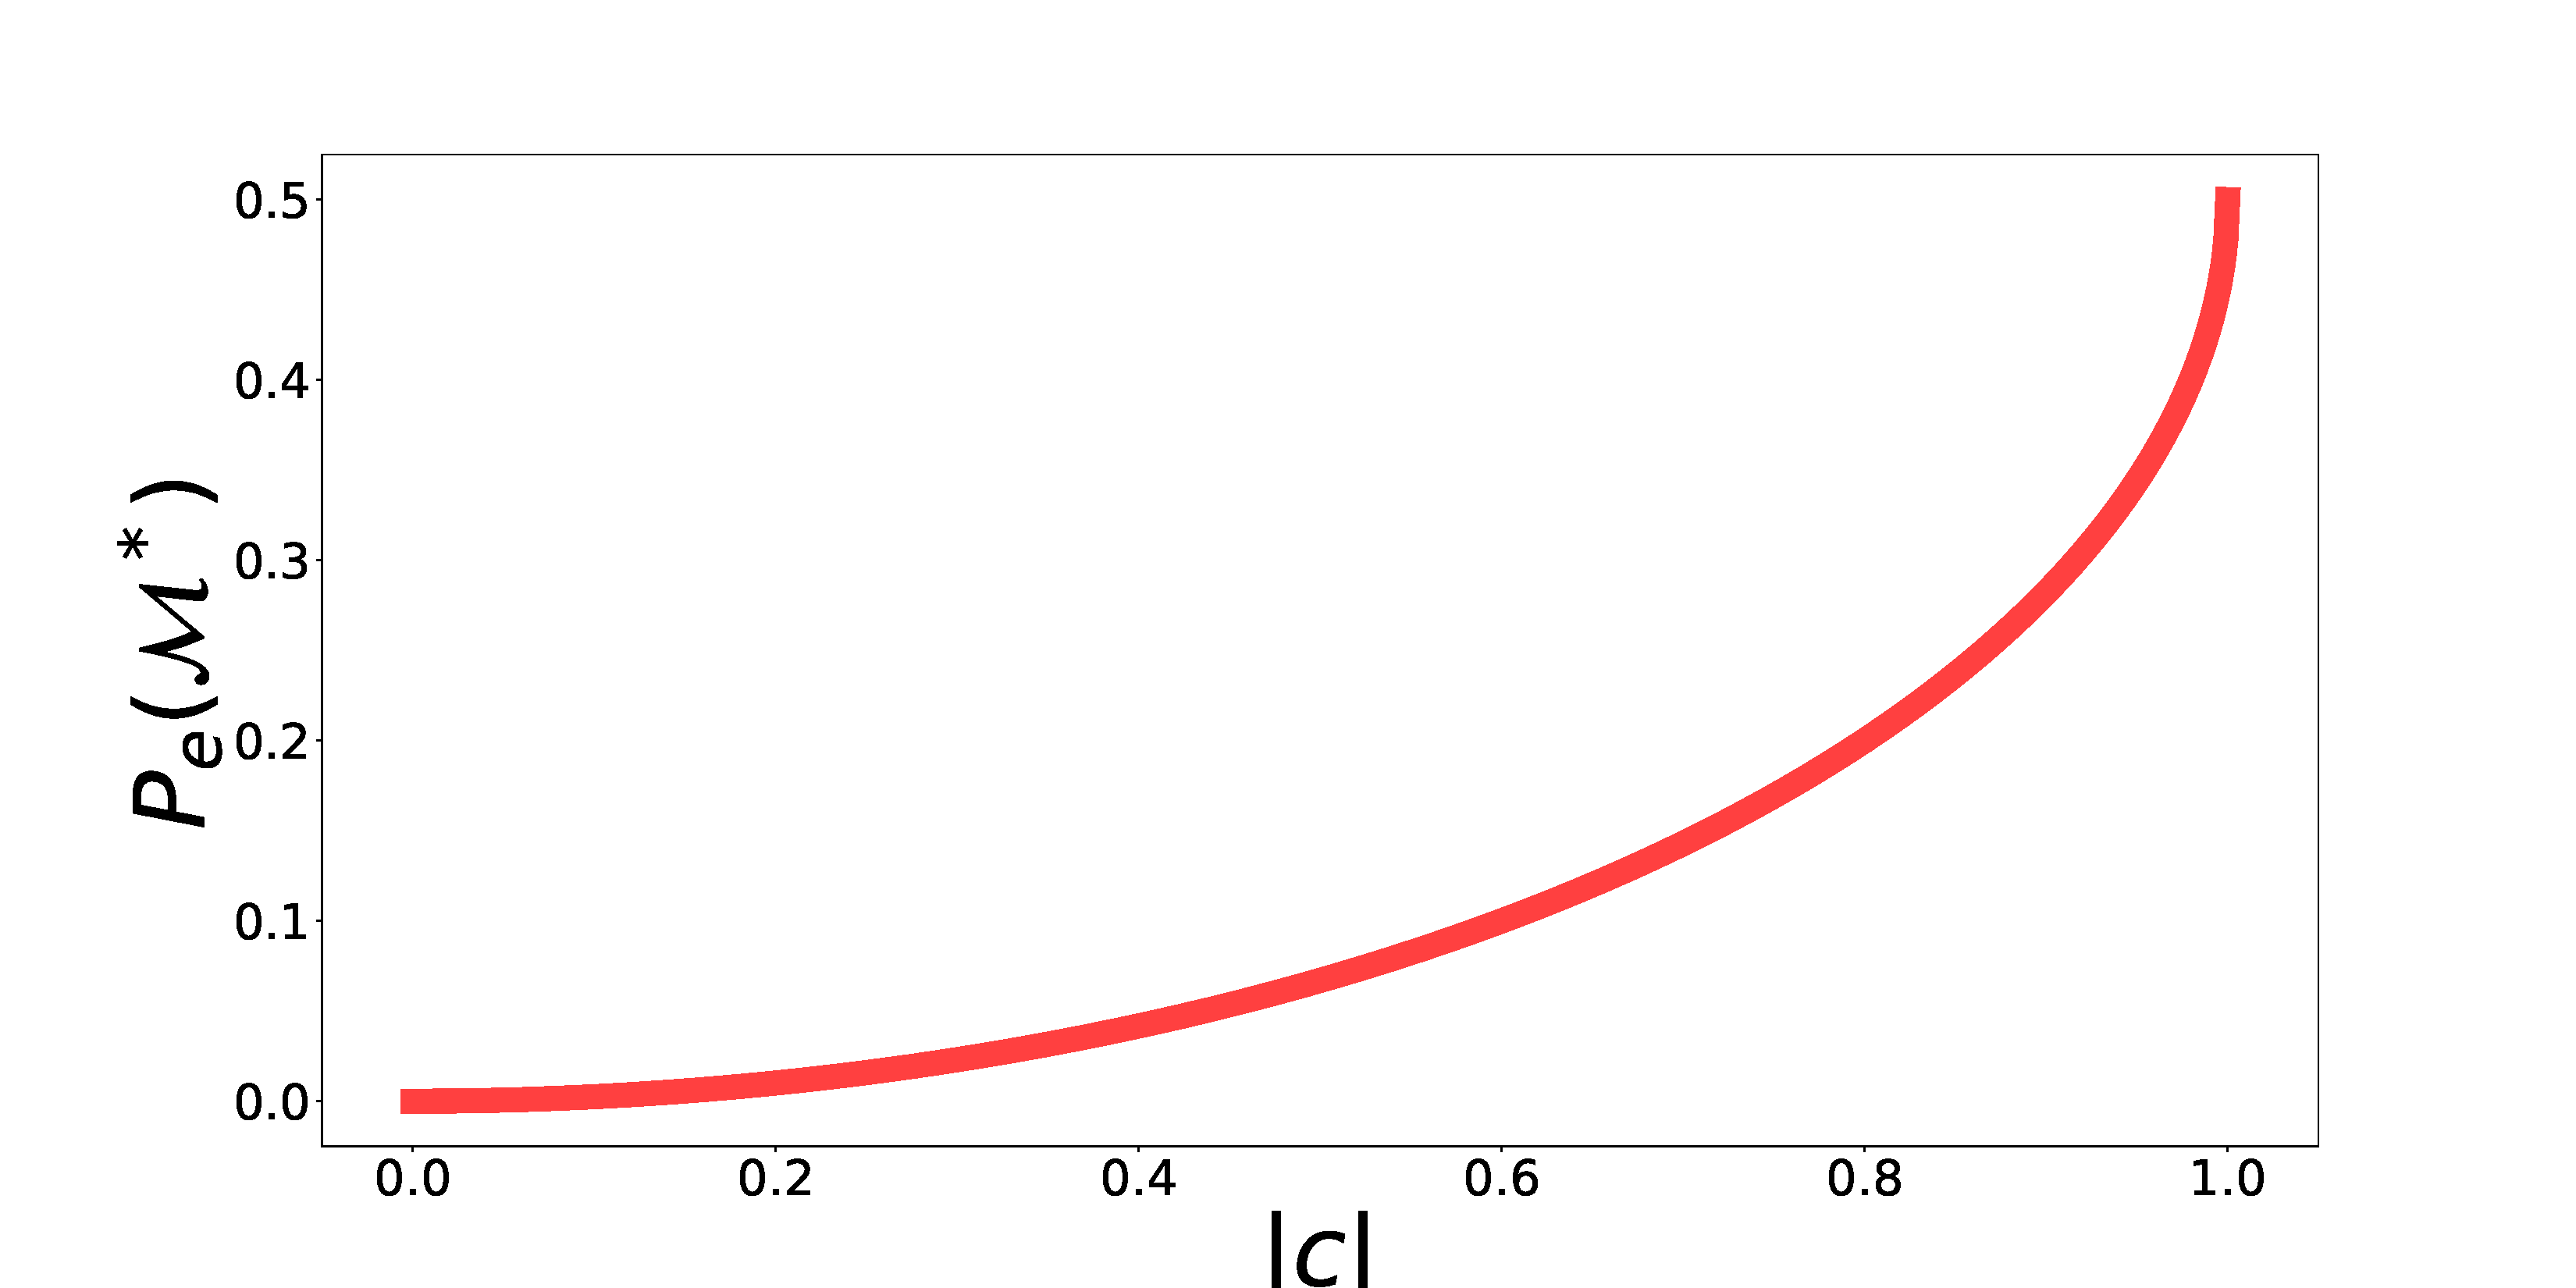
\includegraphics[width=1.\textwidth]{Figures/117/helstrom.pdf}
    \caption{We show Helstrom bound for the error probability when discriminating between two pure states as a function of their overlap $c$ (aboslute value).}
    \label{fig:helpure}
\end{figure}

To sum up, we have discussed the basics of single-shot quantum state discrimination; long is the road that continues this discussion. For instance, we ommited unambiguous state discrimination, where we demand that every time we guess for one hypothesis no errors are commited. This requires that we allow an extra \textit{I don't know outcome}, that deems that data inconclusive; in such case we are interested in minimizing the probability associated to such inconclusive outcome.

Also, we have not discussed multiple-hypothesis problems. In particular, closed-form solutions are known if the states are generated by a symmetry group; here, the optimal POVM is the \textit{pretty-good} (or square-root) measurement, and can be obtained explicitely in terms of the candidate states. In the non-symmetric case, such measurement often provides a \textit{pretty-good} success probability~\cite{Wooters1994prettygood, CrokeReviewQSD}. Also it is worth mentioning that semidefinite programming~\cite{boyd} will not be discussed here. The latter is a technique that allows to efficiently convex optimization problems (and relates to state discrimination when numerically optimizing over measurements).

%



% \subsubsection{Beyond minimum-error state discrimination}
% \textit{Unambiguous state discrimination} The POVM $\mathcal{M}$ can be constructed in such a way to allow for unambiguous discrimination, at the cost of potentially label outcomes as unconclusive. Here, $\mathcal{M} = \{ M_0, M_1, M_? \}$, and the unconclusive outcome is obtained with probability $p_?(\mathcal{M}) = \sum_{k=0,1} p_k p(?|k)$. For instance, in the case of pure states, we can readily construct the measurement operators as projectors onto orthogonal subpsaces of the states constituing the hypothesis; these are $M_0 = \frac{\proj{\psi_1^\perp}}{1+\braket{\psi_0}{\psi_1}}$ (guesses for $\ket{\psi_0}$),
% $M_1 = \frac{\proj{\psi_0^\perp}}{{1+\braket{\psi_0}{\psi_1}}}$
% (guesses for $\ket{\psi_1}$) and $M_? = \mathbb{I} - M_0 - M_1$ (leading to the unconclusive outcome); note that the accompanying coefficients of the projectors ensure that $M_? \geq 0$. We can readily see that when either outcome 0 or 1 are obtained, the test is conclusive, while a finite probability of unconcluding the test arises. In this setting, the challenge is thus to minimize the probability of undeciding, which is certainly relevant if no errors can be admitted in the discrimination task.
%
% \textit{Multiple-state discrimination $\&$ the Pretty Good Measurement}. We have seen that the optimal measurement in the minimum-error binary discirmination scenario is given by a complicated projection defined by the states to be distinguished. The optimal measurement in the multiple-hypothesis scenario has in general an unknown structure; nonetheless a \textit{pretty good measurement} (or square root measurement) can be derived, which in different scenarios such as symmetric pure states turns out to be optimal. Such approach constructs the optimal measurement from the square root of a mixture between the hypothesis states~\cite{Wooters1994prettygood, CrokeReviewQSD}.
%
% \textit{Semi-definite programming}. The optimization over POVM can be casted as a convex problem, which in turn can efficiently be solved through. Moreover, a dual problem can be formulated, which sometimes allows for analytical solutions (or bounds) useful for the problem at hand. For instance, it has been shown using this technique that the Dolinar-type receivers we consider in Chapter~\ref{chapter:RLCOH} can not be optimal when dealing with more than two hypothesis~\cite{Optimal2018Nakahira}.
%
% \textit{Beyond one-shot discrimination}. Discerning between quantum states is thus a primitive related to the description of physical entities. In its general setting, it is not possible to perfectly distinguish between two states, and either a finite probability of undecision arises, or one seeks for minimum-error strategies. In this thesis, we will focus on the latter. As shown above, the success probability is bounded in the one-shot scenario, but more information can certainly be acquired if more copies of the states are available. In turn, the error probability exponentially decreases with the number of copies, and deriving rates at which it does so is the matter of \textit{quantum hypothesis testing}. For example, in the \textit{i.i.d.} scenario, generalizations of the classical testing framework are known: while the symmetric error decrases with a rate known as the quantum Chernoff coeficient\cite{Audenaert2007Discrimination}, the assymmetric errors have quantum relative entropies as rates~\cite{Hiai1991,Stein2}. In these lines, the optimal measurement attaining such rates might be highly non-local (\textit{i.e.} act globally on all the copies available). Nevertheless, for the case of binary pure state discrimination, it has been shown that one can be assymptotically optimal if measuring locally and bayesian updating the priors~\cite{Acin2005Multi}.
%
% We will now review the framework of (classical) statistical inference, which will serve as a basis for characterizing quantum evolutions from measurement signals in Chapter~\ref{chapter:CMON}.
% \textit{A brief comment about quantum communications}
% What happens if we want to transmit a classical message over a quantum channel? such many information processing tasks depends on it. For instance, when capacity-attaining codes such as polar codes ~\cite{qpcodeswilde} rely on performing Helstrom measurement.


%%%
